% Brief explanation of the Schwarz-Christoffel transform
% David Lawrence Miller
% d.l.miller@bath.ac.uk
 
% Started : 29 October 2008
% Completed (first draft) : 
% Really completed :
 
\documentclass[a4paper,10pt]{amsart}
 
% Load some packages
\usepackage{times, amsmath, amssymb, amsfonts, url, natbib, graphicx, multirow, bm, rotating}
 
\usepackage{multirow}
 
% top matter
\title{The Schwarz-Christoffel transform and its possible application to finite area smoothing}
\author{David Lawrence Miller}
\email{d.l.miller@bath.ac.uk}
\address{Mathematical Sciences, University of Bath, Bath, United Kingdom}
 
% Shortcuts
% Probability
\newcommand{\prob}[1]{\mathbb{P}\left[ #1 \right]}
% Hovitz-Thompson
\newcommand{\HT}{\hat{\tau}_{HT}}
% Schwarz-Christoffel
\newcommand{\sch}{Schwarz-Christoffel }
% fprime
\newcommand{\fprime}{f^\prime(z)}

\begin{document}
 
% The abstract
\begin{abstract}
Smoothing in a complex region is difficult. Current approaches (eg. soap film smoothing, (\cite{soap}, \emph{pp.154-160}) or FELSPLINE (\cite{ramsay}))are computationally expensive. Here we propose a method for using the \sch transform to morph a complex region to a more managable shape in order to smooth over points in it.
\end{abstract}
 
 
% New theorem for theorems
\newtheorem{thm}{Theorem}[section]
 
%New theorem for definitions
\newtheorem{defn}{Definition}[section]
 
\maketitle



\section{Motivation}

It is often the case in ecological modelling that the survey region is not defined by the person analysing the data. Indeed it is often defined by the physical characteristics of the survey region. In this case we find that there are peninulae or irregular edges which are difficult to smooth over. Phenomena such as ``leakage'' occur and, as a result, cause the model to over-estimate density.

\section{Method}

In order to smooth around a complex region, one approach is to transform the shape of the region into a form that is easier to smooth over. So, for example, we could transform a region into a rectangle, circle or other familiar shape to avoid the problems found in (for example) \cite{ramsay}. To do this we wish to find some mapping between the original and transformed region (see fig. (\ref{simpledia}).)

% Simple diagram showing the mapping
\begin{figure} [htbp]
\centering
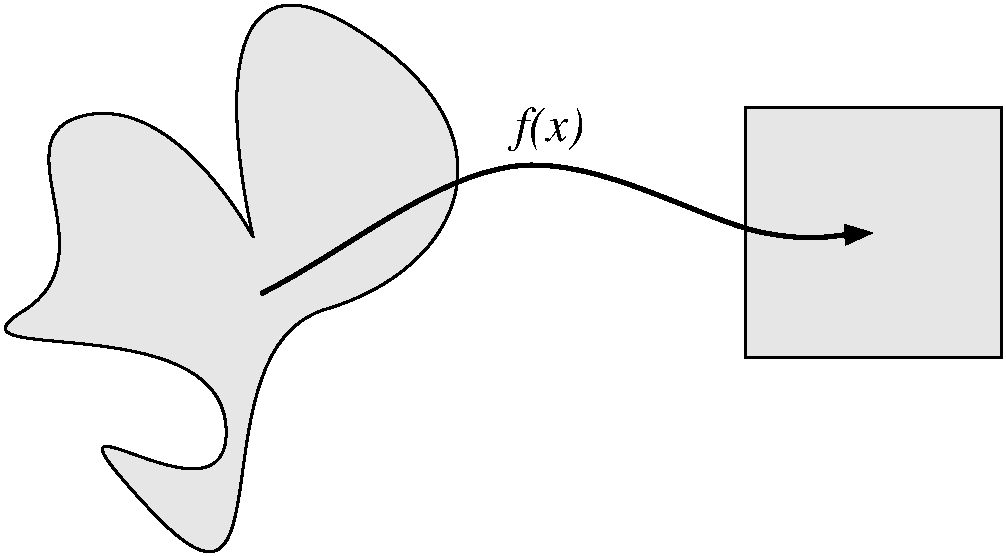
\includegraphics[scale=0.3]{figs/simpledia.pdf}
\caption{The function $f$ takes the points in the rectangle and maps them to the region on the left.}
\label{simpledia}
\end{figure}

In our case we use a method from complex analysis called the \sch mapping. This takes some arbitrary polygon and maps it to the upper half-plane ($H^+$) or the unit disk. This is achieved in the $H^+$ case by taking the vertices of the polygon and mapping them to points on the real line (see fig. (\ref{reallinedia}).) For the unit disk case, we look for points on the circle bounding the unit disk and which vertices they map to on the polygon (see fig. (\ref{unitdiskdia}).)

% Diagram showing upper half plane to polygon
\begin{figure} [tbp]
\centering
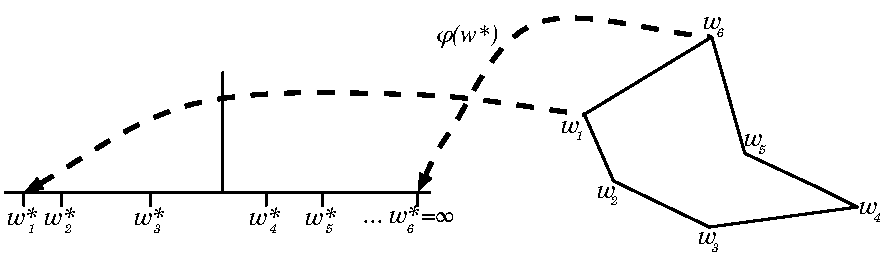
\includegraphics[scale=0.6]{figs/reallinedia.pdf}
\caption{Here we show the mapping of the upper half-plane to the polygon. The vertices ($w_k$) are the result of applying $f$ to the points on the real line ($z_k$). The boundry of the polygon is mapped to the real line.}
\label{reallinedia}
\end{figure}

% Diagram showing unit disk to polygon
\begin{figure} [tbp]
\centering
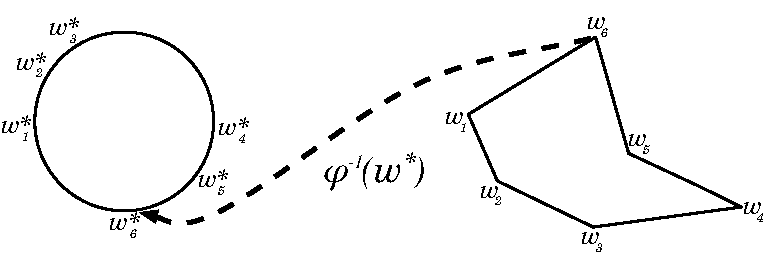
\includegraphics[scale=0.6]{figs/unitdiskdia.pdf}
\caption{We now have the same situation as in fig. \ref{reallinedia}, except that now the boundry of the polygon is mapped to the boundry of the unit disk.}
\label{unitdiskdia}
\end{figure}

Although the \sch mapping is intended for use with polygons, it is easy to take some artibrary region and draw a polygon around it. This can be done either by eye (for example, using the \texttt{locator()} function in \textbf{R}) or by using an automated process.


\subsection{Nomenclature}

We first define a polygon formally and its associated quantities as it will be referred to throughout the rest of the document.

A polygon, $\Gamma$, is a collection of vertices $w_1, w_2,\dots,w_n$ and interior angles $\alpha_1\pi, \alpha_2\pi, \dots, \alpha_n\pi$. For convenience we define $w_{n+1} = w_1$ and $w_0=w_n$. Note that $w_k \in \mathbb{C} \cup {\infty}$. Numbering of vertices is anti-clockwise. The angles are such that $\alpha_k \in (0,2]$ and we require:

\begin{equation}
\sum_{k=1}^n (1-\alpha_k) = 2.
\end{equation}

We also define the exterior angle, $\beta_k\pi$, as given by $(1-\alpha_k)\pi$ (see fig. (\ref{anglediagram}).)

% Diagram showing the exterior/interior angle relationship.
\begin{figure} [bp]
\centering
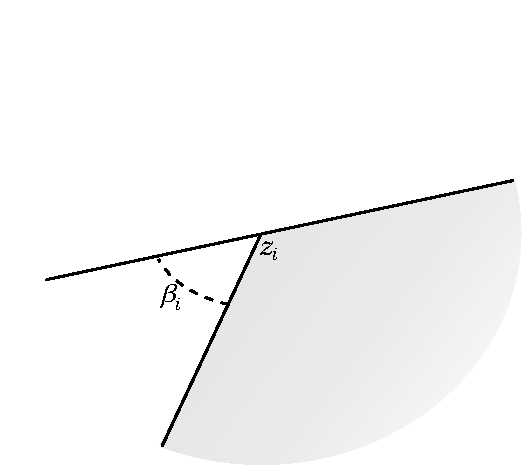
\includegraphics[scale=0.6]{figs/anglediagram.pdf}
\caption{The external angle $\beta_k$ is associated with the vertex $w_k$. The internal angle is given by $\alpha_k$.}
\label{anglediagram}
\end{figure}

Usually, $\Gamma$ is used to refer to the boundary of the polygon and $P$ to the region inside.

Since in the \sch transform we are actually looking for the inverse of the map from the polygon to the plane (or disk). We use the function $f$ to go from the unit disk or $H^+$ to the polygon and the inverse of $f$, $g$ to go from the polygon to the disk or half-plane.  

We need to know the position that the vertices on $\Gamma$ (the $w_k$s) correspond to on the real line (or the boundry of the unit disk). These points are referred to as \emph{prevertices} and are denoted $z_k$.

It is certainly worth noting at this point (to avoid confusion) that those points on the polygon are always referred to as $w_k$ and those on the unit disk or $H^+$ as $z_k$. 

 
\section{\sch Mapping}

We now look at the mathematical formulation for both the upper half-plane and unit disk.

\subsection{Mapping to the upper half-plane}

When we map $\Gamma$ to $H^+$ we set $f(\infty) = w_n$ without any loss of generality. We then have the formula:

\begin{equation}
f(z) = A + C \int^z \prod_{k=1}^{n-1} (\zeta-z_k)^{-\beta_k} d\zeta.
\end{equation}

Here $A$ and $C$ are complex constants determined once the $z_k$ have been calculated. These control the scaling and rotation of the transform.

Although setting $f(\infty) = w_n$ does not make any difference in a mathematical sense, it does mean that the density of the points as they are mapped into $H^+$ is rather odd. Given two points near $w_n$, their spacing on the upper half-plane is huge in comparison to two points near the other vertices. For this reason it is more common to use the unit disk mapping, elaborated upon below. This phenomenon is known as ``crowding'' and is covered at length in \cite{driscoll}. 



\subsection{Unit disk}

For the unit disk we do not fix any points, however note below that the product now runs over all of the prevertices. However, the integrand is simply a constant multiple of the original form. This is merely to avoid problems in the calculation of the branch cuts (\cite{driscoll}, \emph{p. 12}).

\begin{equation}
\label{unitscmap}
f(z) = A + C \int^z \prod_{k=1}^{n} (1 - \frac{\zeta}{z_k})^{-\beta_k} d\zeta.
\end{equation}

As above, $A$ and $C$ are complex constants.

\section{Computation of the \sch mapping}

Since it is generally easier to compute the \sch map to the unit disk rather than to $H^+$ (and, as detailed above, we can avoid crowding.) For that reason we only address mappings from/to the unit disk here. We now detail the process for computing the map.


\subsection{Outline of the computation of the map}
To compute the map, we need to find the prevertices, $z_i$\footnote{Since the complex constants just control scaling and rotation, we can compute them after computing the $z_k$.}. We achieve this by approximating the $z_i$ then mapping those points back to the polygon to give an estimate of $\Gamma$, $\Gamma^\prime$. 

In our algorithm we require the following information: 

\begin{enumerate}
\item $w_1, \dots, w_n$, the vertices of $\Gamma$,
\item $n$, the number of vertices,
\item $\beta_1, \dots, \beta_n$, the external angles of $\Gamma$.
\end{enumerate}

It is worth noting that given the vertices, the other two quantities can be easily calculated.

We express this wish in the form of the following set of equations:

\begin{equation}
\label{optimizeme}
\frac{\vert g(z_{k+1}) -  g(z_k) \vert}{\vert g(z_2)-g(z_1)\vert} - \frac{\vert w_{k+1} - w_k\vert}{\vert w_2 - w_1\vert} = 0, \qquad \text{for } k=3,\dots,n-1,
\end{equation}

where $g=f^{-1}$. 

Intuitively we are looking at the differences between the side lengths of the polygon and the polygon as it is estimated by this iteration (\cite{snider}, \emph{p. A-3}), both scaled by the distance between the first two vertices.

Note that the relation does not include the vertex $w_n$, nor do we look at $w_1$ or $w_2$ in the numerator on the right of the above equation. This is since (by theorem 3.1 of \cite{driscoll} \emph{p. 24}) a polygon is precisely defined by its angles and its vertices not including $w_n$\footnote{Since we know the direction of the edges leacving $w_1$ and $w_{n-1}$, we may find the point where they meet.}. We may find the scaling factor, $C$, from (\ref{unitscmap}) by using the following equation:

\begin{equation}
C=\frac{\vert g(z_2)-g(z_1)\vert}{\vert w_2 - w_1\vert},
\end{equation}

otherwise, we can assume that up to scaling and rotation that $w_1$ and $w_2$ are correct. In this case we know that $\Gamma$ and $\Gamma^\prime$ are similar (in the geometric sense.) 


\subsection{Technical details of the computation}

The function $g$ in (\ref{optimizeme}) is found by taking the inverse of $f$, that is:

\begin{equation}
g(z) = \int_{z_j}^{z_{j+1}} f(\zeta) d\zeta.
\end{equation}

Calculating the above integral is time consuming, luckily we may use the Gauss-Jacobi quadrature in order to quickly compute the result. The quadrature is given by:

\begin{equation}
\int_{-1}^{1} (1-x)^\alpha (1+x)^\beta f(x) dx = \sum_{i=0}^{n-1}h_if(x_i) + \epsilon_n,
\end{equation}

where the $h_i$s are weights and the $x_i$ are referred to as nodes. $\epsilon_n$ is an error term. The integral is rescaled to be over the correct interval (\cite{trefethen}, \emph{p. 11}).

Using this, we iterate over the prevertices, calculating the differences between the true and estimated values of the $w_j$s until convergence has been reached.


\subsection{Sketch of an algorithm to calculate the \sch mapping}

\begin{enumerate}
\item Accept inputs:
   \begin{enumerate} 
      \item $w_1,\dots,w_n$ (the vertices),
      \item $n$ (the number of vertices),
      \item $\beta_1,\dots,\beta_n$ (the external angles at each vertex).
   \end{enumerate}
\item Initialise the Gauss-Jacobi quadrature.
\item Define the objective function, $F$, as:
 \begin{equation*}
 F(k,z_1,z_2) = \frac{\vert g(z_{k+1}) -  g(z_k) \vert}{\vert g(z_2)-g(z_1)\vert} - \frac{\vert w_{k+1} - w_k\vert}{\vert w_2 - w_1\vert}, \qquad \text{for } k=3,\dots,n-1,
 \end{equation*}
\item Until $\vert F(k,z_1,\dots,z_n)\vert < \epsilon \quad \forall k$:
\begin{enumerate}
  \item Calculate $F(k,z_1,\dots,z_n) \quad \forall k$:
  \item Change the values of prevertices.
\end{enumerate}
\item Calculate $C$ and $A$.
\item Return values for $z_1,\dots,z_n$, $C$ and $A$.
\end{enumerate}



\subsection{Getting between the polygon and unit disk}

\subsubsection{Forwards map}

Calculating the forwards map is simply a case of evaluating $f$ at the necessary points. For clarity if we wish to find the point on polygon ($w$) given we know the point on the disk ($z$) we compute:

\begin{equation}
\label{unitscmap}
w=f(z) = w_0 + C \int_{z_0}^{z} \prod_{k=1}^{n} (1 - \frac{\zeta}{z_k})^{-\beta_k} d\zeta,
\end{equation}

where $z_0$ is any point in the closed disk such that $w_0 = f(z_0)$ is known and non-infinite. We may choose any point since the integrand is analytic throughout the mapping and hence the integral is path-independent (\cite{driscoll} \emph{p. 27}).


\subsubsection{Backwards map}

To calculate points from the polygon to points on the unit disk, we treat the equation $g(z)=w$ as a non-linear equation to be solved for $z$ (\cite{trefethen}, \emph{pp. 16-17}). These are solved iteratively as a series of first order ODEs, with the starting values coming from inverting (\ref{unitscmap}).

\textbf{SIMON: I know I need to expand on this, but I am waiting for the book to arrive in the library.}

\section{Examples of the mapping}

Using the Fortran library \texttt{SCPACK}\footnote{available at \url{http://www.netlib.org/conformal/sclib} and \url{http://www.netlib.org/conformal/scpack}.}, some wrapper code was written to interface with \textbf{R}\footnote{Code available at \url{http://github.com/dill/phd-smoothing/tree/master}.}

\subsection{The \sch mapping for a sqaure}
We first took a square with vertices at $(10,0), (0,10),(-10,0),(0,-10)$ and mapped this into the unit disk. We then took a regular grid of points and mapped their positions in the unit disk. The results from this can be seen in fig. (\ref{squaredomain}).

% Square domain mapping diagram
\begin{figure} [bp]
\centering
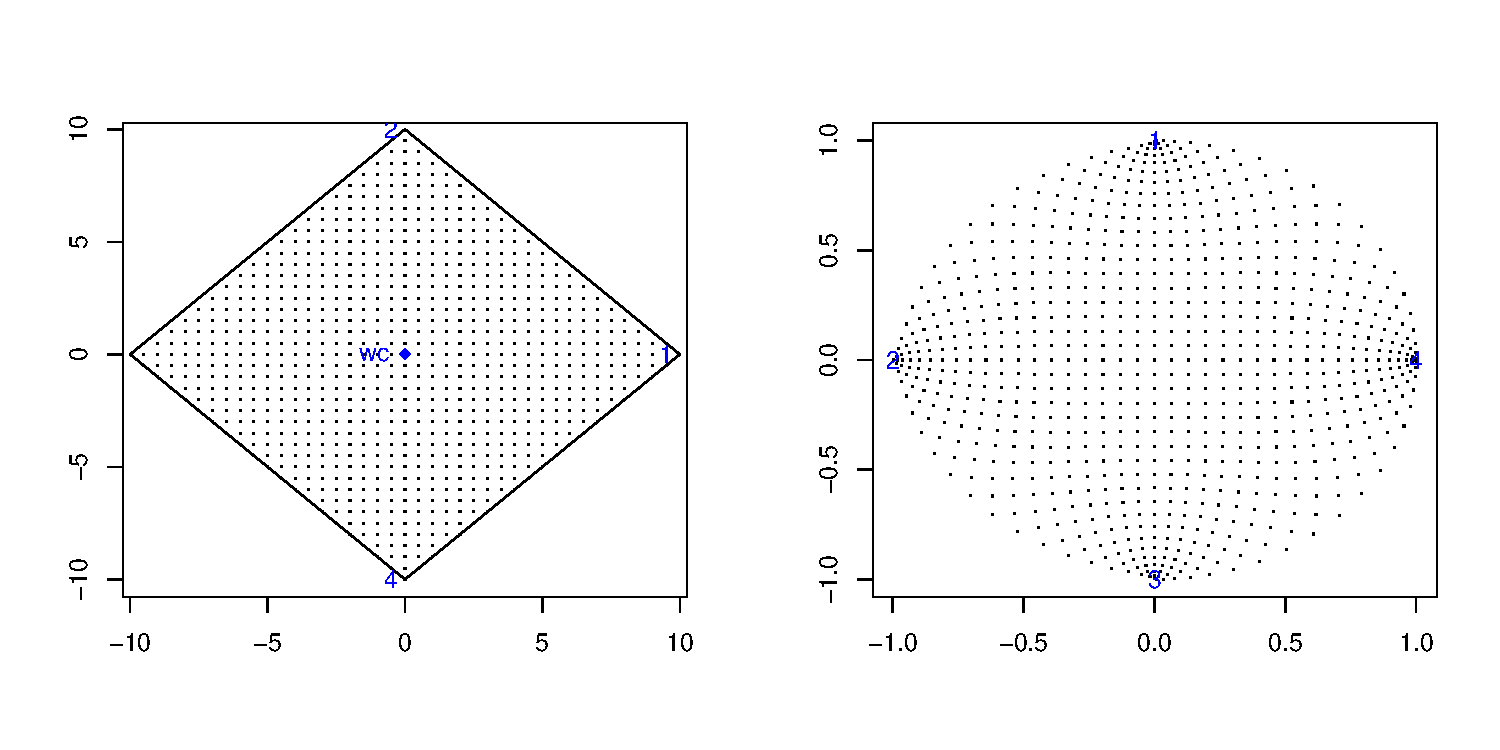
\includegraphics[scale=0.5]{figs/squaredomain.pdf}
\caption{The left panel shows a regular grid of points over the square region. The right panel shows the mapping of these points under the \sch tranformation to the unit disk.}
\label{squaredomain}
\end{figure}

\subsection{An irregular mapping}
Next we used the \textbf{R} function \texttt{locator()} and drew and arbitrary polygon and then mapped this to the unit disk. Then, as above we took a regular grid over the polygon and mapped those points into the disk. The results may be seen in fig. (\ref{irregdomain})


% Square domain mapping diagram
\begin{figure} [tbp]
\centering
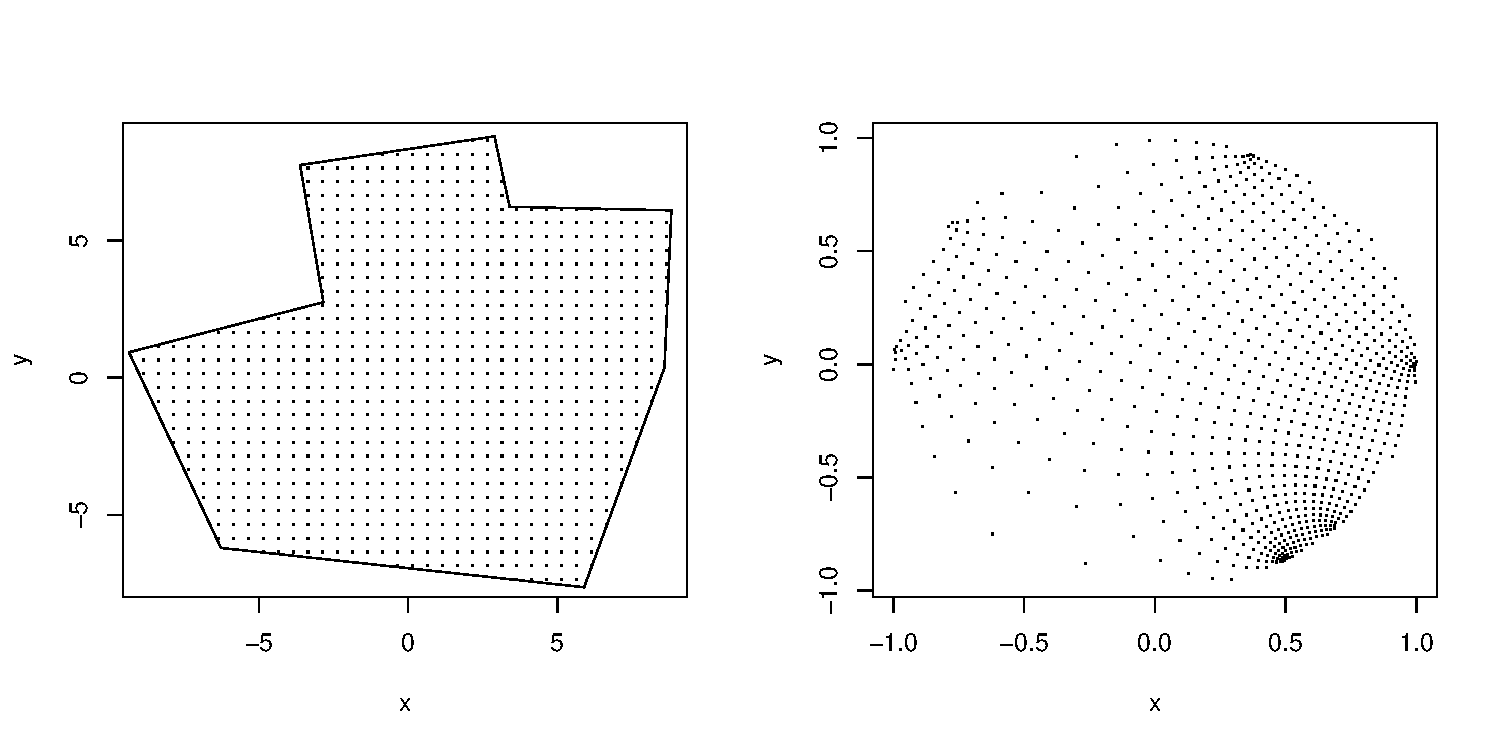
\includegraphics[scale=0.5]{figs/irregulardomain.pdf}
\caption{The left panel shows a regular grid of points over region bound by a irregular nonagon. The right panel shows the mapping of these points under the \sch tranformation to the unit disk.}
\label{irregdomain}
\end{figure}


%\section{Application to finite area smoothing}

%Given some complex geographical area, it is possible to find a polygonal ``bounding box'' that may be fed into the \sch formula. We would then have the region transformed into the  unit disk which would not include any peninsula or other geographical features which are hard to smooth over.

%Once $f$ is found, it would simply be a case of feeding all calculations through it to find the transformed co-ordinates on the unit disk. Once the smooth has been fit the area could be back-transformed and then the smooth used as usual.



\bibliographystyle{plainnat}
\bibliography{sc-refs}

\end{document}
